\documentclass[twoside]{article}
\setlength{\oddsidemargin}{0.25 in}
\setlength{\evensidemargin}{-0.25 in}
\setlength{\topmargin}{-0.6 in}
\setlength{\textwidth}{6.5 in}
\setlength{\textheight}{8.5 in}
\setlength{\headsep}{0.75 in}
\setlength{\parindent}{0 in}
\setlength{\parskip}{0.1 in}
\usepackage{amsmath,amsfonts,graphicx}

\newcounter{lecnum}
\renewcommand{\thepage}{\arabic{page}}
\renewcommand{\thesection}{\arabic{section}}
\renewcommand{\theequation}{\arabic{equation}}
\renewcommand{\thefigure}{\arabic{figure}}
\renewcommand{\thetable}{\arabic{table}}

\newcommand{\lecture}[4]{
   \pagestyle{myheadings}
   \thispagestyle{plain}
   \newpage
   \setcounter{lecnum}{#1}
   \setcounter{page}{1}
   \noindent
   \begin{center}
   \framebox{
      \vbox{\vspace{2mm}
    \hbox to 6.28in { {\bf 15-859: Information Theory and Applications in TCS
		\hfill Carnegie Mellon University} }
       \vspace{4mm}
       \hbox to 6.28in { {\Large \hfill Lecture #1: #2  \hfill} }
       \vspace{2mm}
       \hbox to 6.28in { {\hfill March 26, 2013 \hfill} }
       \vspace{2mm}
       \hbox to 6.28in { {\it Lecturer: #3 \hfill Scribe: #4} }
      \vspace{2mm}}
   }
   \end{center}
   \markboth{Lecture #1: #2}{Lecture #1: #2}
}
%
% Convention for citations is authors' initials followed by the year.
% For example, to cite a paper by Leighton and Maggs you would type
% \cite{LM89}, and to cite a paper by Strassen you would type \cite{S69}.
% (To avoid bibliography problems, for now we redefine the \cite command.)
% Also commands that create a suitable format for the reference list.
\renewcommand{\cite}[1]{[#1]}
\def\beginrefs{\begin{list}%
        {[\arabic{equation}]}{\usecounter{equation}
         \setlength{\leftmargin}{2.0truecm}\setlength{\labelsep}{0.4truecm}%
         \setlength{\labelwidth}{1.6truecm}}}
\def\endrefs{\end{list}}
\def\bibentry#1{\item[\hbox{[#1]}]}

%Use this command for a figure; it puts a figure in wherever you want it.
%usage: \fig{NUMBER}{SPACE-IN-INCHES}{CAPTION}
\newcommand{\fig}[3]{
			\vspace{#2}
			\begin{center}
			Figure #1:~#3
			\end{center}
	}

\newcounter{tnum}
\newtheorem{theorem}{Theorem}[tnum]
\newtheorem{lemma}[tnum]{Lemma}
\newtheorem{proposition}[tnum]{Proposition}
\newtheorem{claim}[tnum]{Claim}
\newtheorem{corollary}[tnum]{Corollary}
\newtheorem{definition}[tnum]{Definition}
\newtheorem{remark}[tnum]{Remark}
\newtheorem{example}[tnum]{Example}
\newenvironment{proof}{{\bf Proof:}}{\hfill\rule{2mm}{2mm}}


\newcommand\E{\mathbb{E}}
\newcommand\ul{\underline}
\newcommand\pow[1]{\mathcal{P} \left( #1 \right)}
\newcommand\size{\operatorname{size}}

\begin{document}
%\lecture{**LECTURE-NUMBER**}{**DATE**}{**LECTURER**}{**SCRIBE**}
\lecture{16}{Monotone Formula Lower Bounds via Graph Entropy}
        {Mahdi Cheraghchi}{Shashank Singh}
%\footnotetext{These notes are partially based on those of Nigel Mansell.}
\vspace{-0.2in}
\section{Recap}
\begin{itemize}
\item {\bf Graph Entropy:} Given $G = (V,E)$, we define $H(G) = \min (X;Y)$
over joint distributions $(X,Y)$, where $X \in V$ is uniformy random and
$X \in Y \subseteq V$. We showed Graph Entropy obeys the following:
\begin{itemize}
\item {\bf Sub-additivity:} $H(G_1 \cup G_2) \leq H(G_1) + G(G_2)$.
\item {\bf Monotonicity:} If $G_1 \subseteq G_2$, then $H(G_1) \leq G(G_2)$.
\item {\bf Disjoint Union:} If $G_1,\dots,G_k$ are the connected components if
$G$, then $H(G) = \sum_i \frac{|V(G_i)|}{|V(G)|} H(G_i)$.
\end{itemize}
\item Last time, we applied Graph Entropy to lower bound the size of
\begin{itemize}
\item a covering of a graph by bipartite graphs
\item a perfect family of hash functions
\end{itemize}
\end{itemize}

\vspace{-0.3in}
\section{Monotone Formula Lower Bounds via Graph Entropy}
\vspace{-0.1in}
Today we examine an application of Graph Entropy to Circuit Complexity.
\vspace{-0.1in}
\subsection{Monotone Boolean Functions}

\begin{definition}
A \ul{boolean function} is one mapping $\{0,1\}^n \rightarrow \{0,1\}$.
\end{definition}
\vspace{-0.2in}
\begin{remark}
We can equivalently consider boolean functions as mapping
$\pow{[n]} \rightarrow \{0,1\}$, using the obvious bijection between
$\{0,1\}^n$ and $\pow{[n]}$. Boolean functions are represented by (not
necessarily unique) boolean formulae or trees in which leaves variables and
internal nodes are logical connectives. We use these representations
interchangeably.
\end{remark}
\vspace{-0.2in}
\begin{definition}
A boolean function $f : \pow{[N]} \rightarrow \{0,1\}$ is \ul{monotone} if
$S \subseteq T \in \pow{[n]}$ implies $f(S) \leq f(T)$. Furthermore, if
$f$ is a monotone boolean function, then the \ul{min-terms of $f$ of size $i$}
are
\[(f)_i
    \buildrel\triangle\over =
        \{S \in \pow{[n]} : |S| = i, f(S) = 1,
                            \mbox{ and } \forall T \subseteq S, f(T) = 0\},
    \quad (f)
        \buildrel\triangle\over =
            \bigcup_{i = 1}^{n} (f)_i.\]
Furthermore, a boolean formula is \ul{monotone} if it contains only AND and OR
connectives.
\end{definition}
\begin{example}
\normalfont
The following are monotone boolean functions:
\begin{enumerate}
\item OR: $x \vee y = 0 \Leftrightarrow x = y = 0$. The min-terms of OR are
$(OR)_1 = \{\{0\},\{1\}\}$, $(OR)_i = \emptyset$ for $i \neq 1$.
\item AND: $x \wedge y = 1 \Leftrightarrow x = y = 1$. The min-terms of AND are
$(AND)_2 = \{\{0,1\}\}$, $(AND)_i = \emptyset$ for $i \neq 2$.
\item MAJ$_3$: $MAJ_3(x_1, x_2, x_3)
    = (x_1 \wedge x_2) \vee (x_1 \wedge x_3) \vee (x_2 \wedge x_3)$.
\end{enumerate}
%TODO: insert tree figures here!
\begin{figure}[h]
\begin{center}
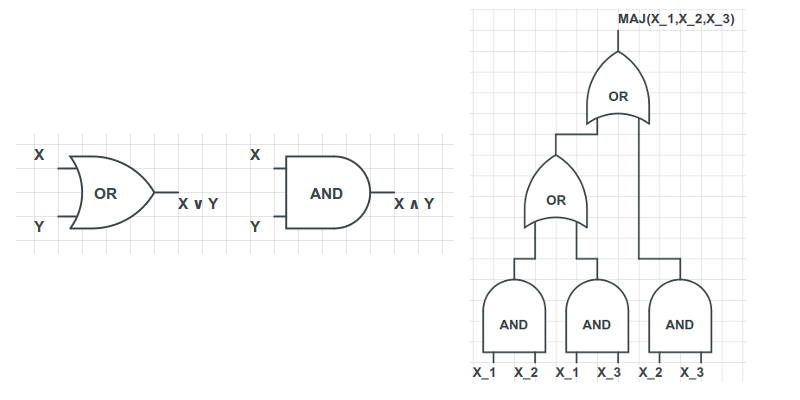
\includegraphics[width=0.8\textwidth]{circuits.png}
\end{center}
\caption{Tree representations of AND, OR, and MAJ$_3$}
\label{fig:2a1}
\end{figure}
\end{example}

\begin{proposition}
A boolean function is monotone iff it can be represented by a monotone boolean
formula.
\end{proposition}

\begin{proof}
Clearly, monotone boolean formulae compute monotone boolean functions.

Let $f$ be a monotone boolean function. Then, $W \subseteq \pow{[n]}$,
$F(W) = 1$ if and only if $\exists S \in (f)$ with $S \subseteq W$. It follows
that $f$ is defined uniquely by $(f)$ as follows:
\[f(x_1,\dots,x_n)
    = \bigvee_{S \in (f)} \left( \bigwedge_{j \in S} x_j \right), \quad
                                    \forall (x_1,\dots,x_n) \in \{0,1\}^n .\]
Note that this formula, called the Disjunctive Normal Form (DNF) of $f$, is
also represented by a binary tree, since many-input logic gates can be
simulated by (linearly many) two-input gates.
\end{proof}

\subsection{Size of a Boolean Function and Threshold Functions}
\begin{definition}
The \ul{size $\size(\phi)$of a formula $\phi$} is the number of nodes in the tree
representation of $\phi$. \\The \ul{size of a boolean function $f$} is
\[ \size(f)
    \buildrel\triangle\over =
        \min_{\phi \mbox{ computing } f} \size(\phi).
\]
That is, $\size(f)$ is number of nodes in the smallest tree computing $f$.
\end{definition}

\begin{definition}
For $k \in [n]$, the \ul{threshold function}
$Th_k^n : \pow{[n]} \rightarrow \{0,1\}$ is defined for $S \in \pow{[n]}$ by
\[ Th_k^n(S)
    \buildrel\triangle\over =
    \left\{
        \begin{array}{cl}
            1 & \mbox{if $|S| \geq k$} \\
            0 & \mbox{else}
        \end{array}
    \right..
\]
\end{definition}

\begin{example}
\normalfont
Threshold functions generalize AND, OR, and MAJ:
\begin{align*}
    AND & = Th_n^n & \size(AND) = 2n - 1 \\
    OR  & = Th_1^n &  \size(OR) = 2n - 1 \\
    MAJ & = Th_{\lceil n/2 \rceil}^n
\end{align*}
It can be shown that MAJ is the `most complex' threshold, in that it
maximizes $\size(Th_k^n)$ over $k$.
\end{example}

\subsection{Bounding the Size of Threshold Functions}
Consider the problem of bounding $\size(Th_k^n)$. For general $k$, the bound
$\size(Th_k^n) \in O(n^{5.3})$ due to (Valiant, 1984) is known, based on a
probabilistic construction which we do not give here.

We analyze the case $k = 2$, for which the following upper bound is easy to
demonstrate:
\begin{claim}
$\size(Th_2^n) \in O(n^2)$.
\end{claim}
\begin{proof}
\[(Th_2^n)_2 = \{\{i,j\} \in \pow{[n]} : i \neq j\}.\]
Furthermore, $\forall i \neq 2$, $(Th_2^n)_i = \emptyset$. Thus, the DNF of
$Th_2^n$ is
\[Th_2^n(x_1,\dots,x_n)
    = \bigvee_{\substack{\{i,j\} \in \pow{[n]} \\ i \neq j}} x_i \wedge x_j,
\]
which (since $\size(AND), \size(OR) \in O(n)$) indicates
$\size(Th_2^n) \in O(n^2)$.
\end{proof}

\begin{remark}
Consider the following Divide and Conquer construction:

Divide the input string $x = (x_1,\dots,x_n) \in \{0,1\}^n$ into
$y = (x_1,\dots,x_{\lceil n/2 \rceil})$ and
$z = (x_{\lfloor n/2 \rfloor},\dots,x_n)$.
Then, we have the recursive formula
\[Th_2^n(x)
    = Th_2^{\lceil n/2 \rceil}(y)
    \vee Th_2^{\lfloor n/2 \rfloor}(z)
    \vee (Th_1^{\lceil n/2 \rceil}(y) \wedge Th_1^{\lfloor n/2 \rfloor}(z)).
\]

This recurrence gives an upper bound: defining $S_n = \size(Th_2^n)$, the
recurrence gives
\[S_n \leq 2S_{n - 1} + O(n),\]
since clearly $\size(Th_1^n) \in O(n)$. The solution of this standard
recurrence (think mergesort) is
\[S_n \leq (2n + \lceil \log n \rceil + 1)(\lceil \log n \rceil)
    \quad \mbox{ and so } \quad
    S_n \in O(n \log n).
\]
\end{remark}

{\bf Exercise:} Refine this bound to
$\size(Th_2^n) \leq 2n \lceil \log n \rceil - 1$. The lower bound we now give
shows this is tight.

We now apply Graph Entropy to prove the lower bound
$\size(Th_2^n) \geq 2 \lceil n \log n \rceil - 1$, following
(Newman, Ragde, and Wigderson 1990).
In order to use graph entropy we're going define a
graph $G_f$ for a boolean function $f$. Consider defining the following:
\begin{definition}
\[G_f \buildrel\triangle\over = (V,E),
    \quad \mbox{where} \quad V \buildrel\triangle\over = [n],
    \quad \mbox{and} \quad
    E \buildrel\triangle\over = (f)_2.
\]
Note that $n$ is from $Th_2^n$ and is not necessarily the number of variables
in $f$.
\end{definition}

\begin{example}
\normalfont
$G_{Th_2^n} = K_n$.
For a single variable $x_i$, $G_{x_i}$ is the empty graph on $n$ vertices.
\end{example}

\newpage
It helps now to have a few lemmas about how graph entropy evolves with AND and
OR operations.

\begin{lemma}
Suppose $f = g \vee h$. Then, $G_f \subseteq G_g \cup G_h$, and hence
$H(G_f) \leq H(G_g) + H(G_h)$.
\label{l:1}
\end{lemma}
\vspace{-0.15in}
\begin{proof}
Suppose $e = \{i,j\} \in E(G_f)$. Then, $1 = f(e) = g(e) \vee h(e)$; without
loss of generality, $g(e) = 1$. By construction of $G_f$, $e \in (f)_2$, so
$f(\{i\}) = f(\{j\}) = 0$. Then, $g(\{i\}) = g(\{j\}) = 0$, so
$e \in (g)_2 = E(G_g)$.
\end{proof}

It would be nice if we also had this property for AND, but it doesn't hold, as
the following example shows:

\begin{example}
\normalfont
Suppose $g(x_1,x_2) = x_1, h(x_1,x_2) = x_2$.
Then, $\{1,2\} \in E(G_f)$, but $\{1,2\} \notin E(G_g), E(G_h)$.
\end{example}

Thus, we need a weaker statement:
\[G_{g \wedge h} \subseteq G_g \cup G_h \cup T_{g,h}.\]

\begin{lemma}
$T_{g,h}$ is the subgraph of $G_f$ induced by edges in
\[ (g)_1 \triangle (h)_1 \buildrel\triangle\over =
((g)_1 - (h)_1) \times ((h)_1 - (g)_1).
\]
\label{l:2}
\end{lemma}
\vspace{-0.3in}
\begin{proof}
Let $e = \{i,j\}$, and let
$f',g',h' : \{0,1\}^2 \rightarrow \{0,1\}$ denote the restrictions of $f,g,h$,
respectively, to $e$ (since the formulae are monotone, we can think of this as
setting the other coordinates to $0$). Then, we have
\[\left.
    \begin{array}{r}
        f'(x_i,x_j) =     x_i \wedge x_j            \\
        g'(x_i,x_j) \neq  x_i \wedge x_j            \\
        h'(x_i,x_j) \neq  x_i \wedge x_j            \\
        f' = g' \wedge h'                           \\
        \mbox{by inspection} \left\{
            \begin{array}{cl}
                g'(x_1,x_2) \neq    x_i \vee x_j    \\
                h'(x_1,x_2) \neq    x_i \vee x_j    \\
            \end{array}
        \right.
    \end{array}
\right\}
\; \Rightarrow \; \mbox{ possible cases are } \; \left\{
            \begin{array}{cl}
                g' = x_i, \quad h' = x_j            \\
                g' = x_j, \quad h' = x_i            \\
            \end{array}
        \right.
\]
(here, we make the simplifying assumption that $f,g,h$ are non-constant
functions; these cases can be analyzed separately) which in turn implies that
$e
    \in ((g)_1 - (h)_1) \times ((h)_1 - (g)_1)
    \buildrel\triangle\over = (g)_1 \triangle (h)_1$.
\end{proof}
\begin{remark}
Since $(g)_1 - (h)_1$ and $(h)_1 - (g)_1$ are disjoint, $T_{g,h}$ is bipartite.
We showed in a previous lecture that this implies $H(T_{g,h}) \leq 1$. Using
subadditivity and the facts
\[
    \begin{array}{rl}
        H(G_{g \vee h})         & \leq H(G_g) + H(G_h)      \\
        H(G_{g \wedge h})       & \leq H(G_g) + H(G_h) + 1  \\
        H(G_{x_i})              & = 0                       \\
        H(G_{Th_2^n}) = H(K_n)  & = \log n,
    \end{array}
\]
we see that any monotone formula for $Th_2^n$ has at least
$\lceil \log n \rceil$ AND gates, and hence
$\size(Th_2^n) \geq \lceil \log n \rceil$.
\end{remark}
We can get an even tighter lower bound by tightening the upper bound on
$H(T_{g,h})$:

Observe that, while $V(T_{g,h}) = [n]$,
$E(T_{g,h}) \subseteq (g)_1 \triangle (h)_1$, which implies, by the disjoint
union property,
\[H(T_{g,h})
    \leq \frac{\left| (g)_1 \triangle (h)_1 \right|}{n}.
\]
Let's define a potential function:
\begin{definition}
\[\mu(f) 
    \buildrel\triangle\over = H(G_f) + \frac{\left| (f)_1 \right|}{n}.
\]
\end{definition}

\begin{claim}
For both $f = g \vee h$ and $f = g \wedge h$, $\mu(f) \leq \mu(g) + \mu(h)$.
\end{claim}
\begin{proof}
Case 1: $f = g \vee h$. Assuming no gate computes a constant function,
\[(f)_1 = \{i : f(\{i\}) = 1\} = (g)_1 \cup (h)_1.\]
Thus,
\[\mu(f)
  = H(G_f) + \frac{\left| (f)_1 \right |}{n}
  \leq H(G_h) + H(G_h) + \frac{\left| (g)_1 \right | + \left| (h)_1 \right|}{n}
  = \mu(h) + \mu(g).
\]
Case 2: $f = g \wedge h$. This time, $(f)_1 = (g)_1 \cap (h)_1$. Thus,
\begin{align*}
\mu(f)
    = H(G_f) + \frac{|(f)_1|}{n}
 &  \leq H(G_h) + H(G_h) + H(T_{g,h}) + \frac{|(g)_1 \cap (h)_1|}{n}        \\
 &  \leq H(G_h) + H(G_h)
        + \frac{|(g)_1 \triangle (h)_1|}{n} + \frac{|(g)_1 \cap (h)_1|}{n}  \\
 &  = H(G_h) + H(G_h) + \frac{|(g)_1| + |(h)_1|}{n}
    = \mu(g) + \mu(h).
\end{align*}

\end{proof}

Note that each leaf has $\mu(x_i) = \frac{1}{n}$ and the root has
$\mu(Th_2^n) = \log n$. Hence, by subadditivity and the preceding claim,
there must be at least $\lceil n \log n \rceil$ leaves. Since each gate has two
inputs and one output, it follows that there are at least
$\lceil n \log n \rceil - 1$ internal nodes, for a total lower bound of
\[\size(Th_2^n) \geq 2\lceil n \log n \rceil - 1.\]
\end{document}
